\documentclass[11pt,twocolumn]{article}
\usepackage{amsmath}
\usepackage{amssymb}
\usepackage{bibentry}
\usepackage{cite}
\usepackage{float}
\usepackage[margin=1in]{geometry}
\usepackage{tikz}
\usepackage[section]{placeins}

\floatstyle{boxed}
\restylefloat{figure}

\usetikzlibrary{arrows,backgrounds,decorations.pathmorphing,positioning}

\newcommand{\comment}[1]{}

\title{Canary}
\author{Andrew Carter}

\begin{document}
\maketitle

\section{Problem Statement}
Determine whether a graph $G$ has a minor isomorphic to $H$.
In particular we consider $G$ to have a minor $H$ if we can find a function $f : H \to 2^G$
 such that for all $h \in H$, $f(h)$ is non-empty and connected,
  and if there is an edge between $h_i$ and $h_j$
 then there exists a $g_k \in f(h_k)$  and $g_j \in f(h_j)$ that are connected.

\section{General Algorithm}
Let $G_k$ be the set of vertices in $G$ that are assigned to $h_k$ (i.e. $G_k = f(h_k)$).

Vertices $g \in G$ may be in one of three states, a vertex may have no constraints, and is therefore considered unassigned.
A vertex maybe be constrained to a specific $G_k$, and are therefore considered assigned to $h_k$.
Or vertices may be constrainted to a binary union of $G_k \cup G_j$,
 and will be referenced as ``may'' be in $G_k$ or ``may'' be in $G_j$.

Start by considering all vertices in $G$ as unassigned.
Go through each vertex $h_k \in H$ and assign it to a vertex in $G$.

Then for each previously assigned vertex $h_j \in H$ that has an edge between $h_j$ and $h_k$ find a path in $G$ that:
\begin{enumerate}
\item Starts at a vertex in $G_j$
\item Through vertices that may be in $G_j$
\item Through vertices that are unassigned
\item Through vertices that may be in $G_k$
\item Ends at a vertex in $G_k$
\end{enumerate}
All vertices on the path that may be in $G_j$ are then put into $G_j$,
  likewise all vertices on the path that may in $G_i$ are then put into $G_i$.
All unassigned vertices on the path are in $G_j \cup G_k$.

Repeat until either the vertices and edges in $H$ are exhausted, or until no path is possible.
If no path is possible backtrack, trying a diffrent path or vertex assignment until all paths and assignments have been tried.


The middle steps may contain $0$ vertices.
Additionally the starting vertex and ending vertex are irrelevant when consider unique paths as they don't affect the change in
 constraints.
\section{Optimizations}
We can apply diffreent optimizations to prevent duplicate or strictly suboptimal paths from being consider.
This prunes the search space, hopefully speeding up termination.

\subsection{Minimal Initial Assignment}
If $h_k$ was assigned to vertex $g \in G$, and then reassigned, then no future assignment need assign $g$ to $h_k$.
\subsection{Minimal Path Length}
If a path has connected vertices $g_j, g_k$ then the path should also contain the edge $g_j, g_k$.

\begin{figure}[H]
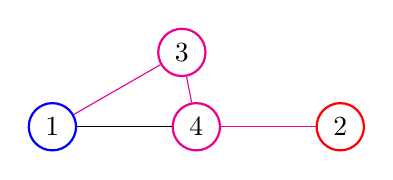
\begin{tikzpicture}
  [
   node distance=5mm and 12mm,
   rn/.style={circle,thick,draw=red,inner sep=0pt,minimum size=6mm},
   gn/.style={circle,thick,draw=green,inner sep=0pt,minimum size=6mm},
   bn/.style={circle,thick,draw=blue,inner sep=0pt,minimum size=6mm},
   yn/.style={circle,thick,draw=yellow,inner sep=0pt,minimum size=6mm},
   cn/.style={circle,thick,draw=cyan,inner sep=0pt,minimum size=6mm},
   mn/.style={circle,thick,draw=magenta,inner sep=0pt,minimum size=6mm}
  ]
   \node[bn] (n1)               {1};
   \node[mn] (n3) [above right=of n1] {3};
   \node[mn] (n4) [right=of n1] {4};
   \node[rn] (n2) [right=of n4] {2};

   \draw[-,color=magenta] (n1) -- (n3);
   \draw[-,color=magenta] (n3) -- (n4);
   \draw[-,color=magenta] (n4) -- (n2);
   \draw[-] (n1) -- (n4);

\end{tikzpicture}
\caption{\label{fig:min path 1.1}Non-Minimal Path}
\end{figure}

In Figure \ref{fig:min path 1.1} we see that the path from 1 to 2 through both 3 and 4 is needlessly long.
We could take the edge directly between 1 and 3, resulting in strictly less constraints.


\subsection{Minimal Path Length on Path Starts}
This can be extended to starting vertices, if vertex $g_j \in G_j$,
  and connected to $g_k$ which is on a path from $G_j$ to $G_k$.
Then the path should contain an edge from a $g \in G_j$ to $g_k$.

\begin{figure}[H]
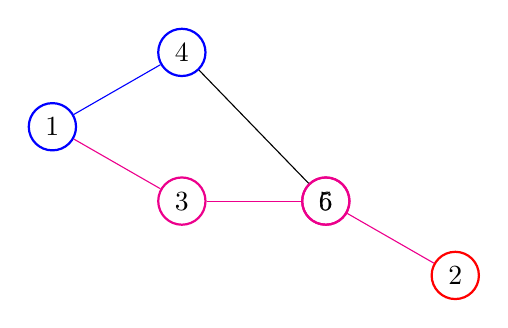
\begin{tikzpicture}
  [
   node distance=5mm and 12mm,
   rn/.style={circle,thick,draw=red,inner sep=0pt,minimum size=6mm},
   gn/.style={circle,thick,draw=green,inner sep=0pt,minimum size=6mm},
   bn/.style={circle,thick,draw=blue,inner sep=0pt,minimum size=6mm},
   yn/.style={circle,thick,draw=yellow,inner sep=0pt,minimum size=6mm},
   cn/.style={circle,thick,draw=cyan,inner sep=0pt,minimum size=6mm},
   mn/.style={circle,thick,draw=magenta,inner sep=0pt,minimum size=6mm}
  ]
   \node[bn] (n1)               {1};
   \node[mn] (n3) [below right=of n1] {3};
   \node[bn] (n4) [above right=of n1] {4};
   \node[mn] (n5) [right=of n3] {5};
   \node[mn] (n6) [right=of n3] {6};
   \node[rn] (n2) [below right=of n6] {2};

   \draw[-,color=magenta] (n1) -- (n3);
   \draw[-,color=blue] (n1) -- (n4);
   \draw[-,color=magenta] (n3) -- (n5);
   \draw[-,color=magenta] (n5) -- (n6);
   \draw[-,color=magenta] (n6) -- (n2);
   \draw[-] (n4) -- (n6);

\end{tikzpicture}
\caption{\label{fig:min path 2.1}Non-Minimal Path}
\end{figure}

In Figure \ref{fig:min path 2.1}, if vertex 4 is already assigned to vertex 1,
 then the path from 1 to 2 through vertices 3, 5, and 6 is needlessly long.
Instead the path could go through 4 (which is already assigned), then directly to 6 and onto 2.
Again this would result in strictly less constraints.


\subsection{Retroactive Minimal Path Length}
Furthermore if $g_j$ is not assigned to $h_j$, but known to be contained in $G_j \cup G_k$,
  then it follows that if $g_k$ is not connected to a vertex in $G_j$ then $g_j \in G_k$.
Otherwise the previous optimization would be violated.

\begin{figure}[H]
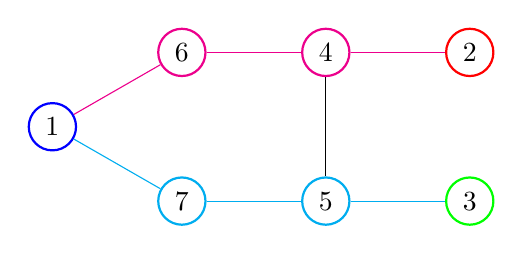
\begin{tikzpicture}
  [
   node distance=5mm and 12mm,
   rn/.style={circle,thick,draw=red,inner sep=0pt,minimum size=6mm},
   gn/.style={circle,thick,draw=green,inner sep=0pt,minimum size=6mm},
   bn/.style={circle,thick,draw=blue,inner sep=0pt,minimum size=6mm},
   yn/.style={circle,thick,draw=yellow,inner sep=0pt,minimum size=6mm},
   cn/.style={circle,thick,draw=cyan,inner sep=0pt,minimum size=6mm},
   mn/.style={circle,thick,draw=magenta,inner sep=0pt,minimum size=6mm}
  ]
   \node[bn] (n1)               {1};
   \node[mn] (n6) [above right=of n1] {6};
   \node[cn] (n7) [below right=of n1] {7};
   \node[mn] (n4) [right=of n6] {4};
   \node[cn] (n5) [right=of n7] {5};
   \node[rn] (n2) [right=of n4] {2};
   \node[gn] (n3) [right=of n5] {3};

   \draw[-,color=magenta] (n1) -- (n6);
   \draw[-,color=magenta] (n6) -- (n4);
   \draw[-,color=magenta] (n4) -- (n2);
   \draw[-,color=cyan] (n1) -- (n7);
   \draw[-,color=cyan] (n7) -- (n5);
   \draw[-,color=cyan] (n5) -- (n3);
   \draw[-] (n4) -- (n5);

\end{tikzpicture}
\caption{\label{fig:min path 3.1}Retroactive Minimal Path Length}
\end{figure}
In Figure \ref{fig:min path 3.1} nodes 1, 2, and 3 are all inital assignments for 3 different vertices in the minor.
 There is a path created between 1 and 2 as shown in magenta through vertices 6 and 4.
 Both vertices may be assigned to either 4 or 6.
 Similarly there is a path between 1 and 3 as shown in cyan through vertices 7 and 5.
\begin{figure}[H]
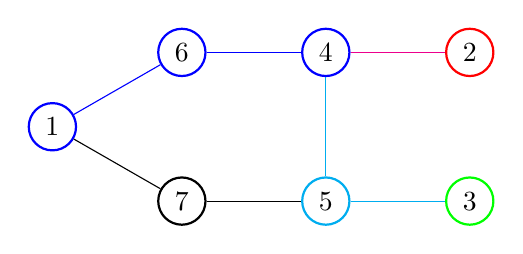
\begin{tikzpicture}
  [
   node distance=5mm and 12mm,
   n/.style={circle,thick,draw=black,inner sep=0pt,minimum size=6mm},
   rn/.style={circle,thick,draw=red,inner sep=0pt,minimum size=6mm},
   gn/.style={circle,thick,draw=green,inner sep=0pt,minimum size=6mm},
   bn/.style={circle,thick,draw=blue,inner sep=0pt,minimum size=6mm},
   yn/.style={circle,thick,draw=yellow,inner sep=0pt,minimum size=6mm},
   cn/.style={circle,thick,draw=cyan,inner sep=0pt,minimum size=6mm},
   mn/.style={circle,thick,draw=magenta,inner sep=0pt,minimum size=6mm}
  ]
   \node[bn] (n1)               {1};
   \node[bn] (n6) [above right=of n1] {6};
   \node[n] (n7) [below right=of n1] {7};
   \node[bn] (n4) [right=of n6] {4};
   \node[cn] (n5) [right=of n7] {5};
   \node[rn] (n2) [right=of n4] {2};
   \node[gn] (n3) [right=of n5] {3};

   \draw[-,color=blue] (n1) -- (n6);
   \draw[-,color=blue] (n6) -- (n4);
   \draw[-,color=magenta] (n4) -- (n2);
   \draw[-] (n1) -- (n7);
   \draw[-] (n7) -- (n5);
   \draw[-,color=cyan] (n5) -- (n3);
   \draw[-,color=cyan] (n4) -- (n5);

\end{tikzpicture}
\caption{\label{fig:min path 3.2}Assigning 4 to vertex 1}
\end{figure}

In Figure \ref{fig:min path 3.2} we see that if we were to assign 4 to vertex 1,
  that there would be a more minimal path from 1 to 3 which does not need to use vertex 7.

\begin{figure}[H]
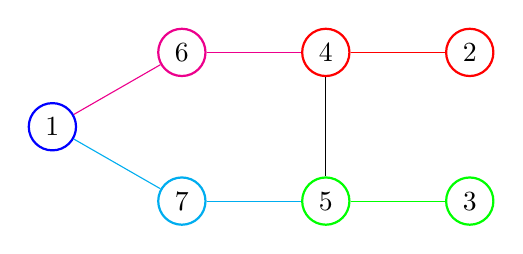
\begin{tikzpicture}
  [
   node distance=5mm and 12mm,
   rn/.style={circle,thick,draw=red,inner sep=0pt,minimum size=6mm},
   gn/.style={circle,thick,draw=green,inner sep=0pt,minimum size=6mm},
   bn/.style={circle,thick,draw=blue,inner sep=0pt,minimum size=6mm},
   yn/.style={circle,thick,draw=yellow,inner sep=0pt,minimum size=6mm},
   cn/.style={circle,thick,draw=cyan,inner sep=0pt,minimum size=6mm},
   mn/.style={circle,thick,draw=magenta,inner sep=0pt,minimum size=6mm}
  ]
   \node[bn] (n1)               {1};
   \node[mn] (n6) [above right=of n1] {6};
   \node[cn] (n7) [below right=of n1] {7};
   \node[rn] (n4) [right=of n6] {4};
   \node[gn] (n5) [right=of n7] {5};
   \node[rn] (n2) [right=of n4] {2};
   \node[gn] (n3) [right=of n5] {3};

   \draw[-,color=magenta] (n1) -- (n6);
   \draw[-,color=magenta] (n6) -- (n4);
   \draw[-,color=red] (n4) -- (n2);
   \draw[-,color=cyan] (n1) -- (n7);
   \draw[-,color=cyan] (n7) -- (n5);
   \draw[-,color=green] (n5) -- (n3);
   \draw[-] (n4) -- (n5);

\end{tikzpicture}
\caption{\label{fig:min path 3.3}Implied Assignments}
\end{figure}
Therefore in the original position we must assign 4 to vertex 2, and likewise 5 is assigned vertex 3 as shown in Figure \ref{fig:min path 3.3}.


% No bibliography, change if/when citations are added
\bibliographystyle{alpha}
\nocite*{}
\nobibliography{bib/main}
\end{document}

